\subsection{Discovery results and pre-specified status}

We report results on two independent splits of the VQA-RAD test set, both run with
identical sample indices for the two models: a \textbf{discovery split} (indices
0000--0099, $n{=}100$ per model, 59 closed-ended questions) on which the metric family
is screened, and a held-out \textbf{confirmation split} (indices 0100--0249, $n{=}150$
per model, 79 closed-ended questions) on which the pre-specified primary test and the
discovery candidates are re-tested. Following our pre-specified protocol
(Section~\ref{sec:hypotheses}), every metric with a Holm-adjusted $p<0.05$ on discovery
is a \emph{discovery candidate}; a candidate is reported as a \emph{finding} only if it
replicates on confirmation ($p_\text{raw}<0.05$, same direction). Both runs are now
complete; Section~\ref{sec:confirmation} reports the confirmation outcome.

\subsection{The pre-specified metric family}

Table~\ref{tab:family} reports all eleven pre-specified metrics, each compared
base-vs-medical per sample with a two-sided Mann--Whitney $U$ test (closed accuracy:
Fisher's exact). Two pairs are deterministic transforms of each other (perplexity of
log-prob; entry depth of entry layer) and carry identical statistics, so the eleven
declared metrics are nine distinct quantities. With Holm--Bonferroni correction across
those nine, \textbf{five distinct effects survive} (Figure~\ref{fig:metric-family}).

\begin{table}[h]
\centering
\caption{Pre-specified metric family, Gemma-3-4B (base) vs.\ MedGemma-4B (medical)
on the discovery split ($n{=}100$). Values are per-sample medians. $|\delta|$ is the
Cliff's delta effect size (Cohen's $h$ for accuracy, marked $^{h}$); with the cut-offs of \citet{romano2006appropriate}:
$|\delta|{<}0.147$ negligible, $|\delta|{<}0.33$ small, $|\delta|{<}0.474$ medium, and larger values large.
$p_\text{raw}$ is the per-sample two-sided Mann--Whitney $U$ (Fisher's exact for
accuracy). Rows marked $\dagger$ are deterministic transforms of the row above them
(perplexity${=}\exp(-$log-prob$)$; entry depth${=}$entry layer${/}$num-layers) and
carry identical statistics, so the eleven declared metrics are \textbf{nine distinct
quantities}; $p_\text{Holm}$ is Holm-adjusted across those nine. \textbf{Five of the
nine survive} ($p_\text{Holm}{<}0.05$). These are the \emph{discovery candidates}
re-tested on the confirmation split (Table~\ref{tab:confirm}). $p_\text{perm}$ is a
two-sided permutation test on the difference of medians (10{,}000 permutations). It has
little power for integer-valued or tied metrics (entry layer, peak layer), where the
Mann--Whitney $p$ is the test of record.}
\label{tab:family}
\begin{tabular}{lcccrrr}
\toprule
\textbf{Metric} & \textbf{Gemma} & \textbf{MedGemma} & $|\delta|$ & $p_\text{raw}$ & $p_\text{Holm}$ & \textbf{$p_\text{perm}$} \\
\midrule
Mean answer log-prob           & $-0.181$ & $-0.256$ & 0.51 & $4.9{\times}10^{-10}$ & $4.4{\times}10^{-9}$ & $\le 10^{-4}$ \\
\quad Answer perplexity $\dagger$ & 1.198 & 1.292 & 0.51 & $4.9{\times}10^{-10}$ & $4.4{\times}10^{-9}$ & $\le 10^{-4}$ \\
First-token entropy            & 0.438  & 0.215  & 0.30 & $2.9{\times}10^{-4}$ & $2.3{\times}10^{-3}$ & 0.0013 \\
Image entry layer              & 11.0   & 11.5   & 0.28 & $5.5{\times}10^{-4}$ & $3.8{\times}10^{-3}$ & 0.117 \\
\quad Image entry depth $\dagger$ & 0.324 & 0.338 & 0.28 & $5.5{\times}10^{-4}$ & $3.8{\times}10^{-3}$ & 0.117 \\
IF AUC (\texttt{image\_to\_last}) & 0.0015 & 0.0007 & 0.26 & $1.6{\times}10^{-3}$ & $9.4{\times}10^{-3}$ & 0.0024 \\
Closed yes/no logit margin     & 10.75  & 7.25   & 0.33 & $1.9{\times}10^{-3}$ & $9.5{\times}10^{-3}$ & 0.013 \\
\midrule
Image peak layer               & 17.0   & 17.0   & 0.19 & 0.017 & 0.067 & 1.0 \\
Question dominance ratio       & 4.96   & 4.02   & 0.19 & 0.019 & 0.067 & 0.053 \\
Closed yes/no accuracy         & 57.6\% & 76.3\% & $0.40^{h}$ & 0.050 & 0.099 & n/a \\
IF Gini (\texttt{image\_to\_last}) & 0.670 & 0.713 & 0.13 & 0.121 & 0.121 & 0.124 \\
\bottomrule
\end{tabular}
\end{table}

\begin{figure}[h]
  \centering
  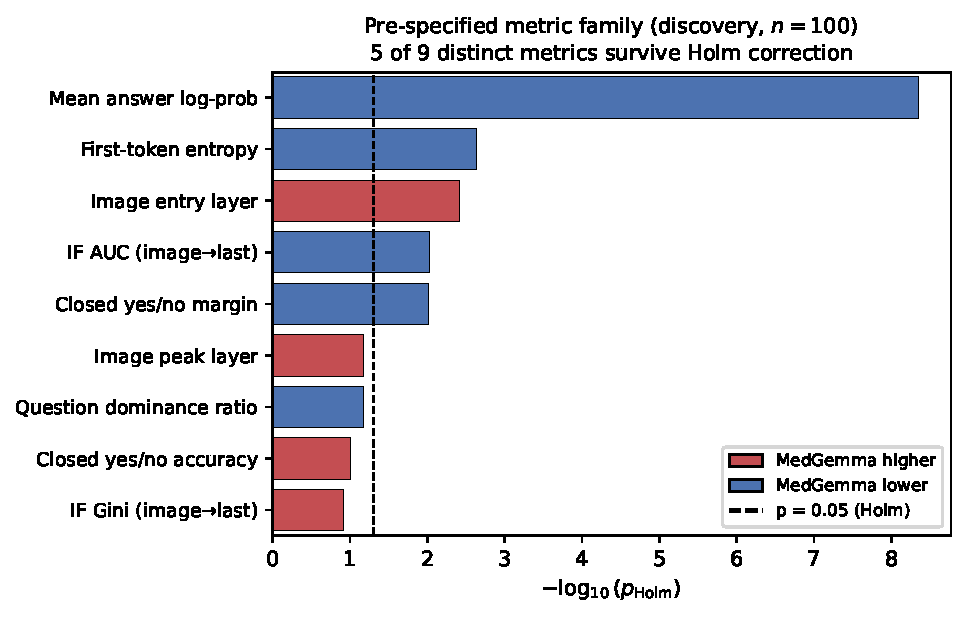
\includegraphics[width=0.82\linewidth]{figures/fig_metric_family}
  \caption{Pre-specified metric family on the discovery split ($n{=}100$). This is the
  \emph{screening} step: by design it is computed on the discovery split only, and its
  candidates are re-tested on the held-out confirmation split in
  Fig.~\ref{fig:confirmation} and Table~\ref{tab:confirm}.
  Bars show $-\log_{10}(p_\text{Holm})$ per metric; the dashed line is the $p{=}0.05$
  significance threshold after Holm correction. Colour indicates direction (red:
  MedGemma higher than Gemma; blue: lower). Shown are the nine distinct quantities
  (the two deterministic-transform aliases are omitted); five survive correction.}
  \label{fig:metric-family}
\end{figure}

\subsection{What survives on the discovery split}

Three of the five surviving discovery effects concern the decoder's use of the image and
its answer confidence, and give a consistent picture of \emph{how} medical fine-tuning
changes decoding. We stress that these are discovery candidates: on the
confirmation split (Section~\ref{sec:confirmation}) first-token entropy holds, IF AUC
holds at the raw level only, and the entry-layer effect is overturned.

\begin{itemize}
  \item \textbf{Image evidence enters later} (entry layer 11.0 $\to$ 11.5; entry
        depth $0.324 \to 0.338$; Cliff's $\delta{=}0.28$, $p_\text{Holm}{=}0.004$).
        The median shift is only half a decoder layer: a small effect size, but a
        highly consistent one \emph{on this split}. Contrary to our H1, the medical
        model begins driving its answer with image information slightly \emph{deeper} in
        the stack, not earlier. \emph{This effect does not replicate on the confirmation
        split} (Section~\ref{sec:confirmation}) and we do not carry it as a finding.
  \item \textbf{Lower image$\to$answer flow} (discovery IF AUC $0.0015 \to 0.0007$;
        $p_\text{Holm}{=}0.009$): summed over layers, the medical model routes
        \emph{less} image information to the answer. Normalised by each model's answer
        probability, the question pathway falls by the same factor (about 0.6), so this is a
        general drop in flow rather than an image-specific shift. This replicates on the confirmation
        split at the raw level (Section~\ref{sec:confirmation}). The per-layer curves
        (pooled, $n{=}250$, descriptive only) are in Fig.~\ref{fig:finetuning-shift}; a normalised-depth
        view is in Fig.~\ref{fig:layer-full}.
  \item \textbf{More decisive first token} (first-token entropy $0.438 \to 0.215$;
        $p_\text{Holm}{=}0.002$): the medical model commits to its answer with
        markedly lower uncertainty.
\end{itemize}

\begin{figure}[h]
  \centering
  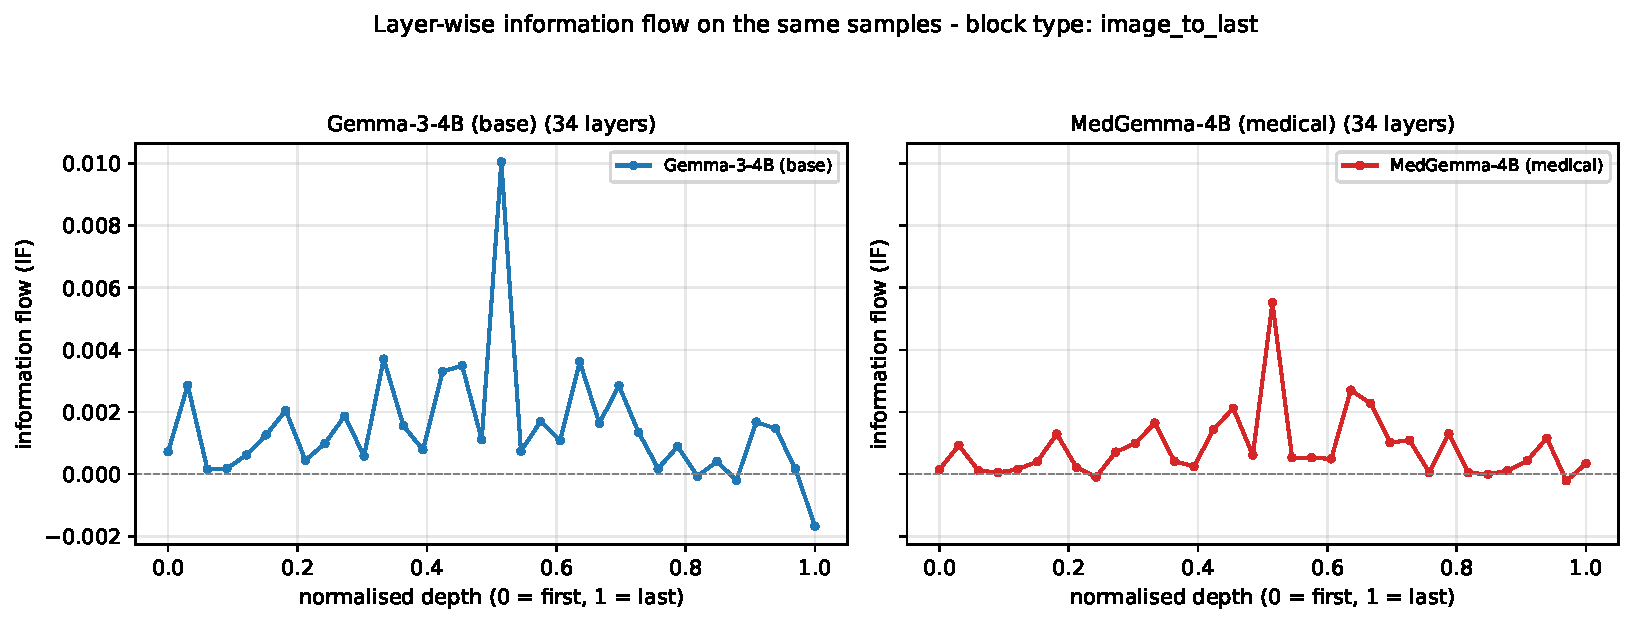
\includegraphics[width=\linewidth]{figures/fig_model_layer_comparison}
  \caption{Per-layer \texttt{image\_to\_last} information flow on a normalised depth
  axis $[0,1]$. Left: Gemma-3-4B (base, blue). Right: MedGemma-4B (medical, red).
  Each curve is the mean over all $n{=}250$ samples (discovery and confirmation pooled;
  descriptive only, computed after the confirmation result was known).
  Both panels share the same y-axis.}
  \label{fig:layer-full}
\end{figure}

\begin{figure}[h]
  \centering
  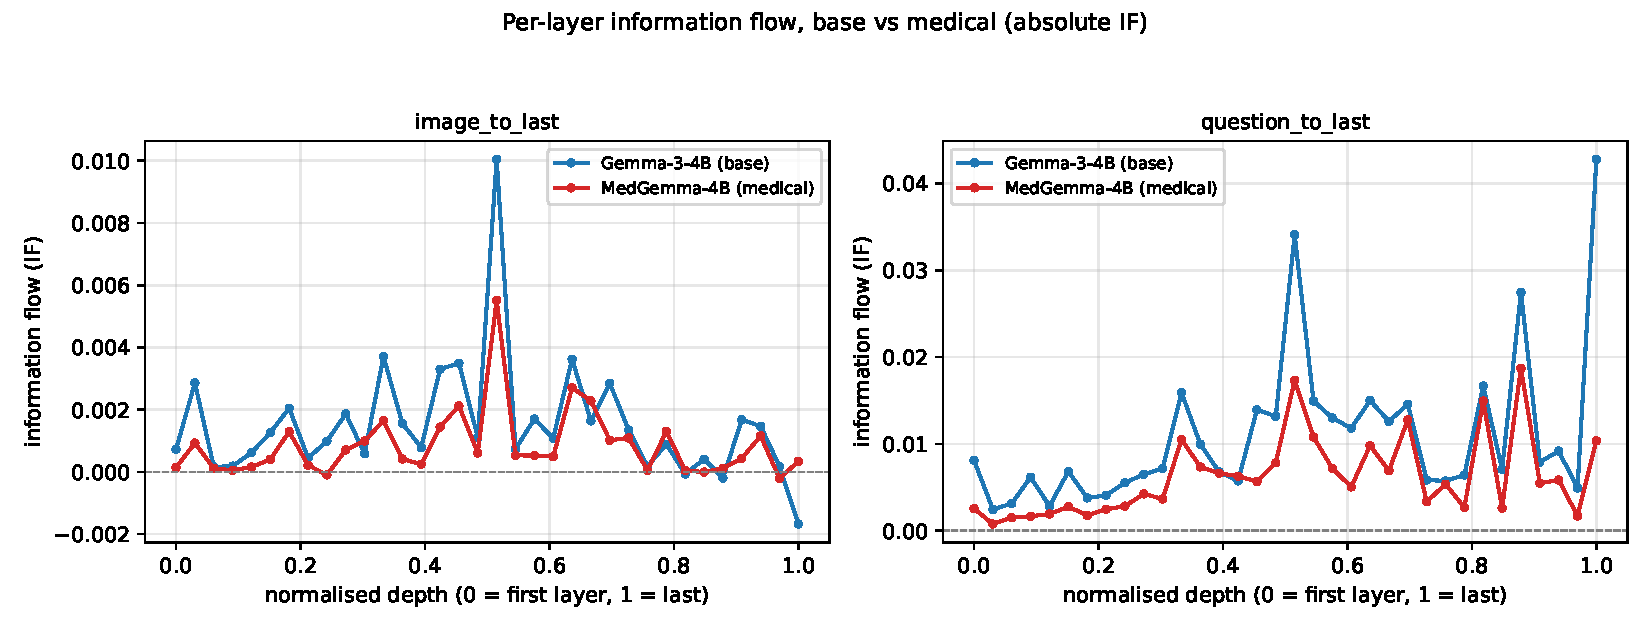
\includegraphics[width=0.85\linewidth]{figures/fig_finetuning_shift}
  \caption{Per-layer information-flow curves (mean over all $n{=}250$ samples, discovery
  and confirmation pooled; descriptive only, no p-values).
  \textbf{Left}: \texttt{image\_to\_last} pathway; \textbf{right}:
  \texttt{question\_to\_last}. Blue: Gemma-3-4B (base); red: MedGemma-4B (medical).
  Integrated over layers, MedGemma's flow is lower in both pathways by a similar factor
  (about 0.6 after normalisation)
  (left panel; per-sample median IF AUC $0.0014 \to 0.0008$ on the pooled set,
  descriptive only). Per-layer values
  are small and change sign across layers, which is why all inference is on per-sample
  distributions (Table~\ref{tab:family}) rather than on the aggregate curve.}
  \label{fig:finetuning-shift}
\end{figure}

The two generation-confidence metrics (answer perplexity and mean answer log-prob)
are the most significant of all, but they describe the answer text rather than the
routing. MedGemma's answers are shorter on average (55 vs.\ 64 generated tokens; 66\%
vs.\ 99\% reach the 64-token cap) and each token is less probable, so we report them
for completeness rather than as routing claims. The closed yes/no logit margin shrinks
($10.75 \to 7.25$; $p_\text{Holm}{=}0.009$), indicating less extreme yes/no logits.

\subsection{What does not survive}

The \textbf{question dominance ratio} (our pre-specified primary metric) moves
in the predicted direction (median $4.96 \to 4.02$, a 19\% drop in the median) but is
only borderline after correction ($p_\text{raw}{=}0.019$, permutation $p{=}0.053$,
$p_\text{Holm}{=}0.067$). We note
that an earlier 50-sample pilot reported a much larger QDR drop; that effect did not
replicate at $n{=}100$ and was sample-size sensitive. Although QDR does not clear Holm
on the discovery split, it is our pre-specified \emph{primary} confirmatory test, and
on the larger confirmation split it attains significance in the predicted direction
(Section~\ref{sec:confirmation}). The \textbf{image peak layer}
is unchanged (L17 for both). \textbf{IF Gini} shows no significant difference.

Against the three directional expectations (recorded in protocol Amendment 4), H1 (earlier image entry) is contradicted
on discovery and does not replicate, H2 (lower QDR) is supported by the confirmed
primary test, and H3 (earlier peak layer) is not supported, since the peak is at L17
for both models.

\subsection{Accuracy}

Closed-ended accuracy rises from 57.6\% (34/59) for Gemma to 76.3\% (45/59) for
MedGemma: a $+18.6$ percentage-point gain of the medical model over the base model
(Cohen's $h{=}0.40$, a small-to-medium effect). For context, an always-``yes'' baseline
scores 52.5\% on these 59 questions, so Gemma sits near that baseline while MedGemma is clearly
above it. The gain is sizeable but, at 59 closed questions, underpowered on discovery:
Fisher's exact $p{=}0.050$ raw, not surviving Holm correction ($p_\text{Holm}{=}0.099$).
The confirmation split resolves this: the gain is larger and clearly significant on the
79 closed questions of indices 0100--0249 (Section~\ref{sec:confirmation}).

\subsection{Encoder representation (descriptive)}

The two models' vision encoders differ substantially. On the same 100 images, the
linear CKA between their layer-0 image features is 0.155 and the mean cosine
similarity is 0.33; the first-answer-token distribution shifts by a Jensen--Shannon
divergence of 0.21 nats. The encoder change is therefore large and documented, but
whether the routing changes above are \emph{caused} by the encoder or by the decoder
cannot be separated from these correlational traces (Section~\ref{sec:discussion}).

\subsection{Confirmation split}
\label{sec:confirmation}

We re-ran both models on the held-out confirmation split (indices 0100--0249,
$n{=}150$ per model, 79 closed-ended questions), analysed with the same per-sample
tests and the pre-specified direction. Table~\ref{tab:confirm} reports the primary
test, every discovery candidate, and closed accuracy.

\begin{table}[h]
\centering
\caption{Confirmation split (indices 0100--0249, $n{=}150$ per model; 79 closed-ended
questions). Values are per-sample medians; $|\delta|$ is Cliff's delta.
$p_\text{raw}$ is the two-sided Mann--Whitney $U$ (Fisher's exact for accuracy).
The primary QDR test is evaluated on its own at $\alpha{=}0.05$ (no correction, per
pre-specified protocol). For the discovery candidates, $p_\text{Holm}$ is Holm-adjusted
across the five distinct candidates tested here. $p_\text{perm}$ is the permutation test
on the difference of medians, as in Table~\ref{tab:family}. A candidate is \emph{confirmed} if
$p_\text{raw}<0.05$ in the discovery direction.}
\label{tab:confirm}
\resizebox{\textwidth}{!}{%
\begin{tabular}{lcccrrrl}
\toprule
\textbf{Metric} & \textbf{Gemma} & \textbf{MedGemma} & $|\delta|$ & $p_\text{raw}$ & $p_\text{Holm}$ & \textbf{Verdict} & \textbf{$p_\text{perm}$} \\
\midrule
\multicolumn{8}{l}{\emph{Pre-specified primary test}} \\
Question dominance ratio       & 5.36 & 4.15 & 0.18 & $6.4{\times}10^{-3}$ & n/a & confirmed & 0.003 \\
\midrule
\multicolumn{8}{l}{\emph{Discovery candidates}} \\
Mean answer log-prob           & $-0.176$ & $-0.242$ & 0.51 & $3.0{\times}10^{-14}$ & $1.5{\times}10^{-13}$ & confirmed & $\le 10^{-4}$ \\
First-token entropy            & 0.505 & 0.092 & 0.47 & $3.0{\times}10^{-12}$ & $1.2{\times}10^{-11}$ & confirmed & $\le 10^{-4}$ \\
Closed yes/no logit margin     & 11.25 & 7.75 & 0.26 & $4.4{\times}10^{-3}$ & $1.3{\times}10^{-2}$ & confirmed & 0.005 \\
IF AUC (\texttt{image\_to\_last}) & 0.0014 & 0.0009 & 0.14 & $3.7{\times}10^{-2}$ & 0.074 & raw only & 0.086 \\
Image entry layer              & 11.0 & 11.0 & 0.05 & 0.434 & 0.434 & not replicated & 1.0 \\
\midrule
\multicolumn{8}{l}{\emph{Accuracy (descriptive)}} \\
Closed yes/no accuracy         & 44.3\% & 77.2\% & $0.69^{h}$ & $3.9{\times}10^{-5}$ & n/a & n/a & n/a \\
\bottomrule
\end{tabular}%
}
\end{table}

\begin{figure}[h]
  \centering
  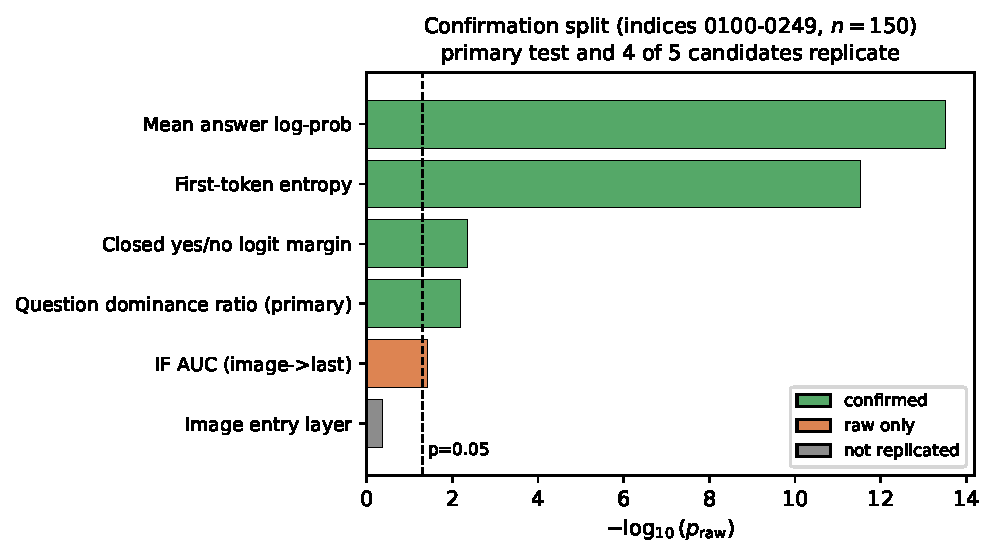
\includegraphics[width=0.78\linewidth]{figures/fig_confirmation}
  \caption{Confirmation split (indices 0100--0249, $n{=}150$ per model). Bars show
  $-\log_{10}(p_\text{raw})$ for the pre-specified primary test (question dominance
  ratio) and the five distinct discovery candidates; the dashed line is the $p{=}0.05$
  replication threshold. Green: confirmed (the primary test, and the three candidates that also survive
  Holm across the five candidates); orange: replicates at the raw level only; grey: not replicated. The primary test and
  four of five candidates clear the threshold in the discovery direction; IF AUC (orange)
  is the one that holds at the raw level only.}
  \label{fig:confirmation}
\end{figure}

\paragraph{Outcome.} The pre-specified \textbf{primary test passes}: the per-sample
question dominance ratio is lower for MedGemma than for Gemma
($5.36 \to 4.15$, Mann--Whitney $p{=}0.006$; permutation $p{=}0.003$; median
95\% CIs $[4.85, 5.91]$ and $[3.66, 4.79]$), in the predicted direction. Under the
pre-specified decision rule, the routing difference between base and medical models is
\emph{confirmed}: relative to its language prior, the medical model relies less on the
question text. Of the five distinct discovery candidates, \textbf{four replicate} at
$p_\text{raw}<0.05$ in the discovery direction (answer log-prob/perplexity, first-token
entropy, closed logit margin, and IF AUC), and \textbf{three of these also survive}
Holm correction across the candidate set; IF AUC replicates at the raw level but not
after correction. The \textbf{image entry layer does not replicate} (median 11.0 for
both models, $p{=}0.43$): the half-layer ``enters later'' shift seen on discovery is not
a reliable effect, and we do not report it as a finding. On closed accuracy the medical
model scores far higher: Gemma 44.3\% vs.\ MedGemma 77.2\% (Cohen's $h{=}0.69$,
Fisher $p{=}3.9{\times}10^{-5}$). This gap should be read with care: on these 79
questions the majority class is ``no'' (55.7\%) and an always-``yes'' response scores
44.3\%, so Gemma (whose forced-choice verdict is ``yes'' for $85\%$ of questions) sits \emph{at} the
always-``yes'' baseline and \emph{below} the majority baseline, while MedGemma is
clearly above both. Part of the $+32.9$-point model-vs-model gap is therefore a baseline
artifact of the base model performing at a trivial level; the defensible statement is
that the medical model clears the majority baseline by $21.5$ points whereas the base
model does not clear it at all.

\paragraph{What the accuracy numbers measure.} The closed-question verdict is a
forced-choice readout. It compares the probability mass on ``yes'' and ``no'' at the first
answer token (\texttt{score\_closed} in \texttt{attn\_knockout/vlm.py}). It is not the
model's written answer. Generations are capped at 64 tokens and often open with a sentence
such as ``Based on the image\ldots'', so the written answer is often not a clear yes or no.
On the confirmation split, the verdict and the written answer agree on $62\%$ of the
MedGemma answers and $91\%$ of the base answers where the text gives a clear verdict. The
text reading is a keyword rule, so it is descriptive only. On the $58$ MedGemma and $53$
base confirmation answers it can decide, the written answer scores $0.52$ and $0.42$, against
$0.79$ and $0.43$ for the verdict on the same items. The accuracy gain therefore depends
partly on the scoring choice. The accuracy comparison in this paper uses the logit verdict,
which replaced the text-extraction scorer found invalid in the pilot; the written-answer scores
are reported to show how much of the gain depends on that choice.

Pooling both splits (indices 0000--0249, $n{=}250$, 138 closed questions) gives a
$+26.8$-point verdict gain and a QDR median of $5.19 \to 4.09$. These pooled figures are
descriptive only. They were computed after the confirmation result was known, so no
p-value is reported for them and they are not evidence in addition to the confirmation
test.

\paragraph{The QDR effect is a median effect.} The primary statistic is the median of
per-sample QDR, as pre-specified, and that is where the effect lives. The mean of the
same per-sample ratios moves the other way: on confirmation it is $6.6$ (95\% CI
$[5.9, 7.4]$) for Gemma and $7.2$ (95\% CI $[5.9, 8.7]$) for MedGemma, with permutation
$p{=}0.47$. Ratios of the mean per-layer curves are also nearly unchanged ($\approx7.2$
vs.\ $\approx7.3$). The reduction is therefore a shift in the typical sample, not in the
average sample, and it is a modest effect. The claim should be read that way.

\paragraph{Robustness to a stricter threshold.} Our pre-specified decision rule fixes
$\alpha{=}0.05$, and we do not alter it post hoc. As a descriptive robustness check,
however, we note which confirmed effects also clear the more stringent $\alpha{=}0.01$:
the primary test (QDR, $p{=}0.006$) and three of the four confirmed candidates
(answer log-prob, first-token entropy, and the closed logit margin, all
$p{<}0.005$) survive at $0.01$, whereas IF AUC ($p{=}0.037$) does not. IF AUC is thus
the single marginal effect. It meets the pre-specified bar but is robust neither to
Holm correction nor to the stricter threshold, and we report it as confirmed but
weak. All other confirmed effects are stable under both checks.

\paragraph{Unreported raw result.} The image peak layer was not a discovery candidate and
its median is unchanged (L17 for both models). On the confirmation split, however, its
two-sided Mann--Whitney test gives $p_\text{raw}{=}0.039$ (median 17 vs.\ 17, rank-biserial
$0.13$). It does not survive Holm correction across the nine distinct quantities
($p_\text{Holm}{=}0.148$), and it was not a pre-specified hypothesis beyond H3, which
predicted an earlier shift. We report it here for completeness and do not treat it as a
finding. The integer-valued tie structure makes this test coarse (see Table~\ref{tab:family}).
